% Fig. 4.12 / CH4_FIGURE_SPECS.md -- the identity z_{alpha/2} =
%   sqrt(chi^2_alpha(1)) drawn as two panels joined by an arrow: the two
%   symmetric tails of the standard normal, once squared, land on the one
%   right tail of chi^2(1).
% Source: mathstatch4.tex lines 4811-4893, a tabular whose first and third
%   cells hold a tikzpicture each and whose middle cell holds
%   $\xRightarrow[]{~X=Z^2~}$.  CH4_FIGURE_SPECS 3.2 requires the arrow to be
%   drawn into the web figure, since it is what ties the two panels together.
%
%   Left panel (manuscript lines 4813-4854): standard normal density, domain
%   -3:3 at samples=400, xmin=-3.2, xmax=3.2, ymin=0, ymax=0.41, bottom axis
%   line only (axis y line=none), no y tick labels, no axis names.  Three x
%   ticks at -1.96, 0 and 1.96 marked $-z_{\alpha/2}$, $0$ and
%   $z_{\alpha/2}$; gray tails at opacity 0.2 on [-3, -1.96] and [1.96, 3]; a
%   segment dropped to the axis from each of the two points, both at height
%   0.05844094; legend $\mathcal{N}(0,1)$.
%
%   Right panel (manuscript lines 4857-4888): chi^2(1) density, written by the
%   manuscript as the Gamma(1/2, 2) density gammadst(x,0.5,2), domain 0:5 at
%   samples=600, xmin=0, xmax=5.2, ymin=0, ymax=0.5, bottom axis line plus a y
%   axis at x = 0 (axis y line=middle), no y tick labels, no axis names.  Two
%   x ticks at 0 and 3.841459 marked $0$ and $\chi^2_{\alpha}(1)$; a gray tail
%   at opacity 0.2 on [3.841459, 5]; a segment dropped to the axis at 3.841459
%   from height 0.02981946; legend $\chi^2(1)$.
%
% The two densities:
%   N(0,1):     f(x) = 0.39894228 e^{-x^2/2}
%   chi^2(1):   f(x) = 0.39894228 x^{-1/2} e^{-x/2}
% with 0.39894228 = 1/sqrt(2 pi).  These reproduce the two heights the
% manuscript hard-codes: f_{N}(1.96) = 0.05844094 and
% f_{chi^2}(3.841459) = 0.02981946, and 1.96^2 = 3.8416, which is the identity
% the figure is about.
%
% Departures from the manuscript figure, all required by the site specs, and
% the same ones as in tail-identity-t-to-f.tex, so that the two figures of
% this piece read as one pair:
%
% 1. Colour and line width per CH3_FIGURE_SPECS 1: curves and axes in
%    journalink at 0.8pt, tails in journalaccent at fill opacity 0.15 rather
%    than gray at 0.2.
%
% 2. The manuscript's legend entry becomes a label written at the curve
%    itself, per CH2 spec 1.9.  Each label sits in the upper corner the
%    density leaves empty.
%
% 3. The tick label $0$ is set on a second row in both panels.
%
% 4. The chi^2(1) density runs to infinity as x approaches 0, and pgfplots
%    cuts it at ymax; the same cut is made here by starting the curve at
%    x = 0.4188, which is where the density equals 0.5.
%
% 5. The two plot boxes are given the same height, 2.60cm, so that the arrow
%    runs level between them, and the two panels are set at the same scale and
%    the same places as in tail-identity-t-to-f.tex.
%
% Size and type.  Drawing range 6.87cm wide, inside the 9.0cm cap of CH2 spec
% 1.3.  A mark of S pt shows at S x 0.99626 x <display width> / <native width>
% px.  The figure sits inside a topic-proof, which indents the body column by
% 1.1em plus a 2px rule, so a topic-figure--wide there is about 328px on a
% 390px phone.  The smallest mark is the alpha and the 2 of the fraction in
% $z_{\alpha/2}$, at scriptscript size, which \DeclareMathSizes{10}{10}{9}{8}
% holds at 8pt rather than the 5pt of the default math sizes.
\documentclass[tikz,border=2pt]{standalone}
\usepackage{amsmath}
\usepackage{amssymb}
\usepackage{xcolor}
\usetikzlibrary{arrows.meta}
\DeclareMathSizes{10}{10}{9}{8}

\definecolor{journalink}{HTML}{1F1C18}
\definecolor{journalmuted}{HTML}{8A7F72}
\definecolor{journalaccent}{HTML}{9C2D2D}

\newcommand{\stdnorm}[1]{0.39894228*exp(-0.5*(#1)*(#1))}
\newcommand{\chisqone}[1]{0.39894228*pow((#1),-0.5)*exp(-0.5*(#1))}

\begin{document}
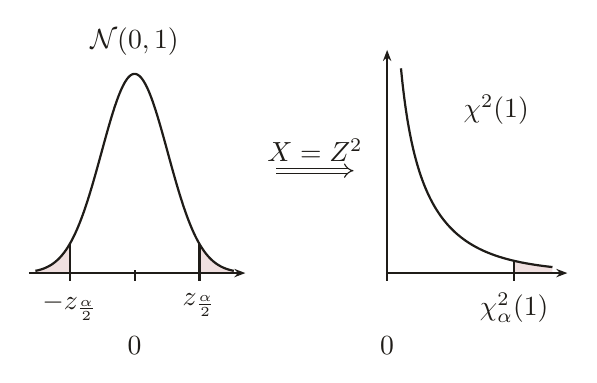
\begin{tikzpicture}[
  x=1cm,
  y=1cm,
  every node/.style={font=\normalsize, journalink},
  axis/.style={journalink, line width=0.8pt, -{Stealth[length=4pt]}},
  tick/.style={journalink, line width=0.8pt},
  curve/.style={journalink, line width=0.8pt},
  drop/.style={journalink, line width=0.8pt},
  tail/.style={journalaccent, fill opacity=0.15}
]
  % ================= left panel: the standard normal ====================
  \begin{scope}[xshift=0cm, x=0.42cm, y=6.34cm]
    \fill[tail] (-3,0) -- (-1.96,0) -- (-1.96,0.05844094)
      -- plot[domain=-1.96:-3, samples=120, smooth] (\x,{\stdnorm{\x}})
      -- cycle;
    \fill[tail] (1.96,0) -- (3,0) -- (3,0.00443185)
      -- plot[domain=3:1.96, samples=120, smooth] (\x,{\stdnorm{\x}})
      -- cycle;

    \draw[curve] plot[domain=-3:3, samples=260, smooth] (\x,{\stdnorm{\x}});

    \draw[axis] (-3.2,0) -- (3.35,0);

    \draw[drop] (-1.96,0.05844094) -- (-1.96,0);
    \draw[drop] (1.96,0.05844094) -- (1.96,0);

    \foreach \p in {-1.96, 0, 1.96}
      \draw[tick] ([yshift=0.035cm]\p,0) -- ([yshift=-0.106cm]\p,0);

    \node[anchor=north, inner sep=0pt] at ([yshift=-0.25cm]-1.96,0)
      {$-z_{\frac{\alpha}{2}}$};
    \node[anchor=north, inner sep=0pt] at ([yshift=-0.25cm]1.96,0)
      {$z_{\frac{\alpha}{2}}$};
    \node[anchor=north, inner sep=0pt] at ([yshift=-0.80cm]0,0) {$0$};

    % Curve label above the peak.  The upper left corner will not hold it:
    % the label is 2.95 units wide, so from x = -3.2 it would run to
    % x = -0.25, where the density has already climbed to 0.387 and would cut
    % through the closing bracket.  Set 0.435 high it clears the peak, 0.3989,
    % by 0.23cm.
    \node[anchor=south, inner sep=0pt] at (0,0.435) {$\mathcal{N}(0,1)$};
  \end{scope}

  % ================= the arrow ==========================================
  \draw[journalink, line width=0.4pt, double, double distance=1.4pt,
        -{Implies[length=5pt]}] (1.80,1.30) -- (2.78,1.30);
  \node[anchor=south, inner sep=2pt] at (2.29,1.34) {$X=Z^{2}$};

  % ================= right panel: the chi-squared density ===============
  \begin{scope}[xshift=3.207cm, x=0.42cm, y=5.20cm]
    \fill[tail] (3.841459,0) -- (5,0) -- (5,0.01464490)
      -- plot[domain=5:3.841459, samples=120, smooth] (\x,{\chisqone{\x}})
      -- cycle;

    % The density passes 0.5, the manuscript's ymax, at x = 0.4188; pgfplots
    % cuts it there and so does this.
    \draw[curve] plot[domain=0.4188:5, samples=320, smooth]
      (\x,{\chisqone{\x}});

    \draw[axis] (0,0) -- (5.45,0);
    \draw[axis] (0,0) -- (0,0.545);

    \draw[drop] (3.841459,0.02981946) -- (3.841459,0);

    \foreach \p in {0, 3.841459}
      \draw[tick] ([yshift=0.035cm]\p,0) -- ([yshift=-0.106cm]\p,0);

    \node[anchor=north, inner sep=0pt] at ([yshift=-0.25cm]3.841459,0)
      {$\chi^{2}_{\alpha}(1)$};
    \node[anchor=north, inner sep=0pt] at ([yshift=-0.80cm]0,0) {$0$};

    % Curve label in the upper right, where the density is below 0.09.
    \node[anchor=west, inner sep=0pt] at (2.3,0.40) {$\chi^{2}(1)$};
  \end{scope}
\end{tikzpicture}
\end{document}
